\chapter{Process Models and System Identification}\label{c:identification}

The following chapter

OUTLINE AND SHORT INTRODUCTION. - System Identification why and why not? Uses and common methods.

Information and so on.

\section{First Order Time Delay Model}%
\label{c:identification:s:fotd}

Information on FOTD / FOPDT process models -> why and why not!?

ORTSKURVEN,NYQUIST ETC.

\section{Graphical Approach} % (fold)
\label{c:identification:s:graphical}

Fedele Approach for Model fitting and show examples!!!

\begin{figure}[H]
\begin{minipage}[b]{\textwidth}
\centering
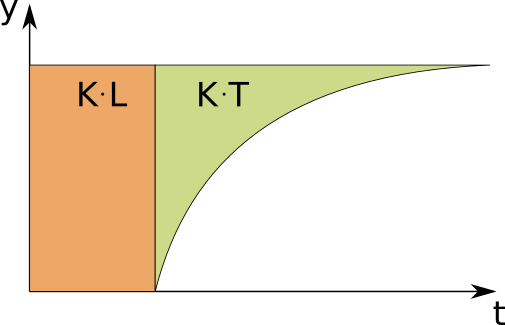
\includegraphics[width=0.9\textwidth]{./Graphics/AREA_IDENTIFICATION1.png}
\caption{Graphical Reprensentation of Identification via Jump Response}
\label{c:control:f:2area}
\end{minipage}
\end{figure}

Probleme: "Überschwinger" -> Wie geanu annähern?

\begin{figure}[H]
\begin{minipage}[b]{\textwidth}
\centering
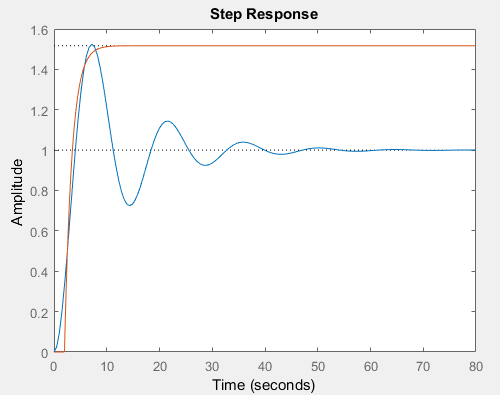
\includegraphics[width=0.9\textwidth]{./Graphics/Overdamped_MATLAB.png}
\caption{Graphical Reprensentation of Identification via Jump Response}
\label{c:control:f:2area}
\end{minipage}
\end{figure}

\begin{figure}[H]
\begin{minipage}[b]{\textwidth}
\centering
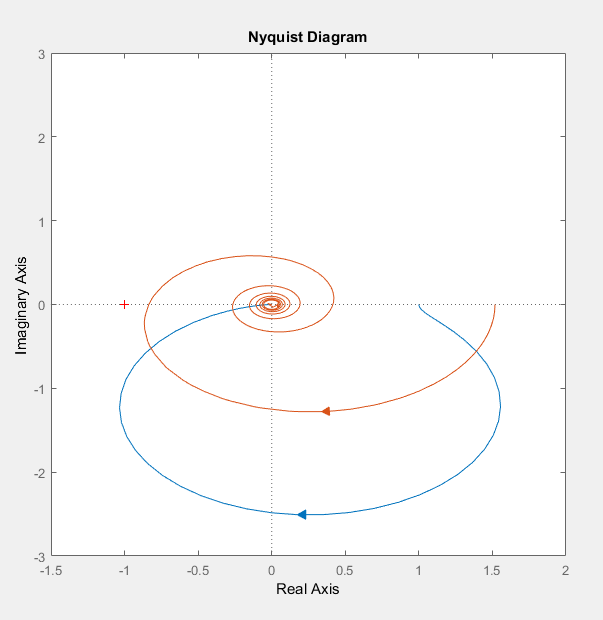
\includegraphics[width=0.9\textwidth]{./Graphics/NYQUIST_MATLAB.png}
\caption{Graphical Reprensentation of Identification via Jump Response}
\label{c:control:f:2area}
\end{minipage}
\end{figure}


\section{Relay Tuning} % (fold)
\label{c:identification:s:relay_tuning}

Relay Tuning for Model fitting

\section{Review and Conclusion}%
\label{c:identification:s:review}

Short review of the results given for both identification processes.
